
\fontsize{12pt}{24pt}\selectfont  (The code for our work can be found at - https://github.com/artshouldterrify/btpsem8)
We used Kaggle notebooks accelerated by a P100 GPU for all model training. 

\section{Dataset}
CIFAKE: Real and AI-Generated Synthetic Images: This dataset comes from two major research works : - Real images are from Krizhevsky \& Hinton (2009)  \cite{7} , fake images are from Bird \& Lotfi (2024)  \cite{6}.  The dataset contains two classes - REAL and FAKE. For REAL, images were collected from Krizhevsky \& Hinton's CIFAR-10 dataset and for the FAKE images, the equivalent of CIFAR-10 with Stable Diffusion Version 1.4 was generated. There are 100,000 images for training (50,000 per class) and 20,000 for testing (10,000 per class). This is the largest dataset of such AI-generated images to date.

\begin{center}
   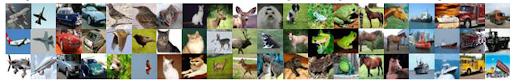
\includegraphics[width=5in,height=1in]{images/4.1.png} 
   \\\fontsize{11pt}{24pt} Figure 4.1: Examples of real images from CIFAR-10 Image Classification Dataset

\end{center}


\begin{center}
   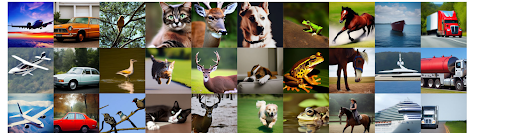
\includegraphics[width=5in]{images/4.2.png} 
   \\\fontsize{11pt}{24pt} Figure 4.2: Examples of AI - Generated images from CIFAKE Dataset
\end{center}



\section{Pre-trained model selection}
In this section, we firstly tested multiple pre-trained models by training and fine-tuning them on 10\% of the dataset. We used a training-testing split of 0.8-0.2 for this portion of the training and we tested models based on ResNet152V2  \cite{19}, NASNetLarge  \cite{25}, DenseNet121  \cite{21} and MobileNetV3Large \cite{28}. We also used a validation set equivalent in size to the testing set, randomly taken from the rest of the dataset. Each of these models uses an input image size of 224x224 and we used 2-neuron dense layer and global 2D-average pooling layer attached to the top of each model with a softmax activation as our classifier. 


We used Keras’ SparseCategoricalCrossentropy as our loss function and the Adam optimizer with an initial learning rate of 0.0001. We also used two callbacks during training, firstly an early stop mechanism stopping training if validation accuracy hasn’t increased for 10 epochs and secondly a learning rate reduction mechanism that reduces the learning if validation accuracy hasn’t improved for 4 epochs. We ran this initial training for 100 epochs per model. After this, we unfroze the top few layers of our base model and fine-tuned the model for another 50 epochs, this time with only the early stopping mechanism and an initial learning rate of 0.00001. 


We input the images directly from the Kaggle notebook’s virtual directory and apply data augmentation using Keras’ preprocessing module. Keras’ ImageDataGenerator utility allows for augmentation to be automatically applied on any data pipeline, allowing for transformations such as rotation, shearing, zoom and vertical/horizontal flips. We used this utility in conjunction with flow\_from\_directory to ultimately create a pipeline that automatically imported data from the virtual directory and simultaneously applied random transformations to it within a set range of parameters that we can define. The parameters we tested for our pipeline are listed in Table 4.1.


    
\begin{table}[H]
\begin{center}
\begin{tabular}{|l|l|l|}
\hline
S.No & Parameter                       & Value \\ \hline
1.   & horizontal flip & True          \\ \hline
2.   & vertical flip      & True          \\ \hline
3.   & rotation range      & 0.5          \\ \hline
4.   & width shift range     & 0.25          \\ \hline
5.   & height shift range     & 0.25          \\ \hline
6.   & shear range     & 0.2          \\ \hline
7.   & zoom range     & 0.4          \\ \hline
\end{tabular}
\end{center}
\caption{Data augmentation parameters}
\end{table}
 
We additionally used the preprocessing\_func parameter of the ImageDataGenerator to apply specific transformations of format that specific pre-trained models required.

\begin{center}
   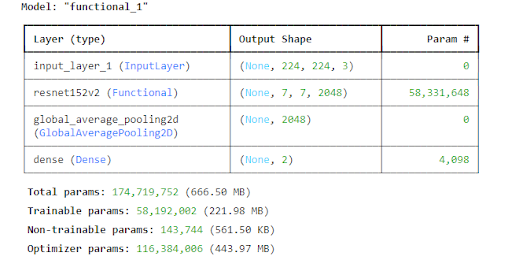
\includegraphics[width=6in,height=3in]{images/4.3.png} 
   \\\fontsize{11pt}{24pt} Figure 4.3: Model Summary
\end{center}

			


We start with the code to define the data input pipeline.
\begin{center}
   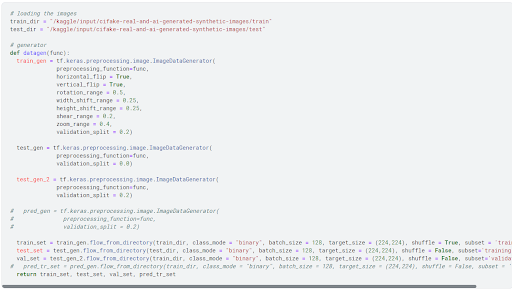
\includegraphics[width=6in,height=5in]{images/c1.png} 
   \\\fontsize{11pt}{24pt} Code: Data pipeline
\end{center}
  
  
We then define the model using Keras’ applications module, which allows us to download pre-trained weights for our base CNNs directly. We define a GlobalAveragePooling2D layer and a 2-neuron softmax Dense layer on top of the model as our classifier.

\begin{center}
   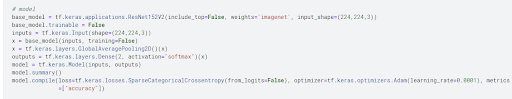
\includegraphics[width=6.5in]{images/c2.png} 
   \\\fontsize{11pt}{24pt} Code: Model definition
\end{center}
  
		
  
We then create instances of the data pipeline, define our callbacks and begin training. 

\begin{center}
   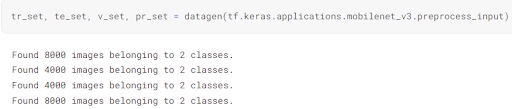
\includegraphics[width=6in]{images/c3.png} 
   \\\fontsize{11pt}{24pt} Code: Pipeline instances
\end{center}

		
\begin{center}
   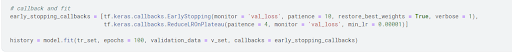
\includegraphics[width=6in,height=1in]{images/c4.png} 
   \\\fontsize{11pt}{24pt} Code: Training
\end{center}
		 

We use the history object created by the .fit function to graph the training process.

\begin{center}
   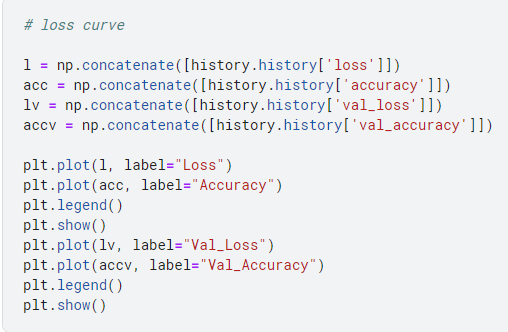
\includegraphics[width=5.5in]{images/c5.png} 
   \\\fontsize{11pt}{24pt} Code: Plotting Training
\end{center}
  
We lastly fine-tuned the model.
\begin{center}
   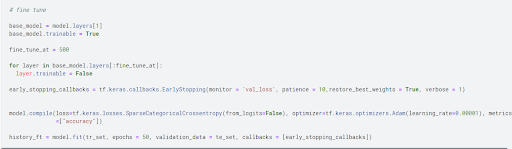
\includegraphics[width=6.5in,height=2in]{images/c6.png} 
   \\\fontsize{11pt}{24pt} Code: Fine Tuning
\end{center}

  
Using this methodology, we trained models based on multiple pre-trained models and accordingly selected the best candidates for our final model. 

\section{Comparison of different metaheuristics}

We picked one of the models trained in section 4.2 and used it to compare different metaheuristic algorithms based on previous comparative studies of metaheuristic algorithms  \cite{13}. For this we used the python library mafese  \cite{28mafese}, a purpose-built library that implements a framework to optimize feature selection problems using multiple methods, including but not limited to metaheuristic algorithms. Mafese is built over another library Mealpy which implements a wide up-to-date range of metaheuristic algorithms. 

To begin, we removed the classifier we had trained over our base CNN (that we picked from the multiple we trained) and processed the same 10\% of the dataset to generate feature representations for training and testing datasets. We then stored these feature representations in a numpy array and define a MhaSelector object, a generalized implementation that allows us to use any metaheuristic we prefer to optimize a generic feature selection problem. This selector trains a separate classifier for any feature subset it explores and outputs the best solution it finds. We iteratively ran this procedure over multiple metaheuristics to find the best algorithm for our data. 

We used a KNN algorithm as our classifier for this step, and we ran each metaheuristic for 50 epochs with a population size of 50. We lastly graphed the results to compare the different algorithms on the number of features selected and the accuracy achieved. 

We start with generating features using our previously defined data pipelines.

\begin{center}
   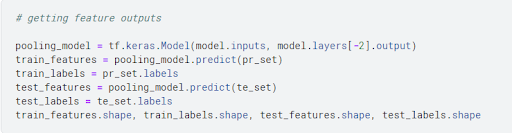
\includegraphics[width=6in,height=2in]{images/c7.png} 
   \\\fontsize{11pt}{24pt} Code: Generating features for metaheuristics
\end{center}

	
 
We then use mafese to iterate over multiple metaheuristics.


\begin{center}
   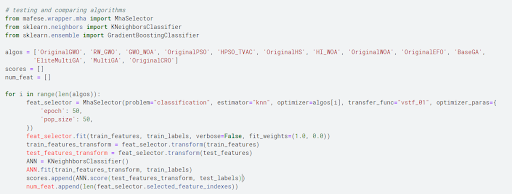
\includegraphics[width=6in,height=3in]{images/c8.png} 
   \\\fontsize{11pt}{24pt} Code: Running metaheuristics
\end{center}

	 
 
We finally plot our results using seaborn.

\begin{center}
   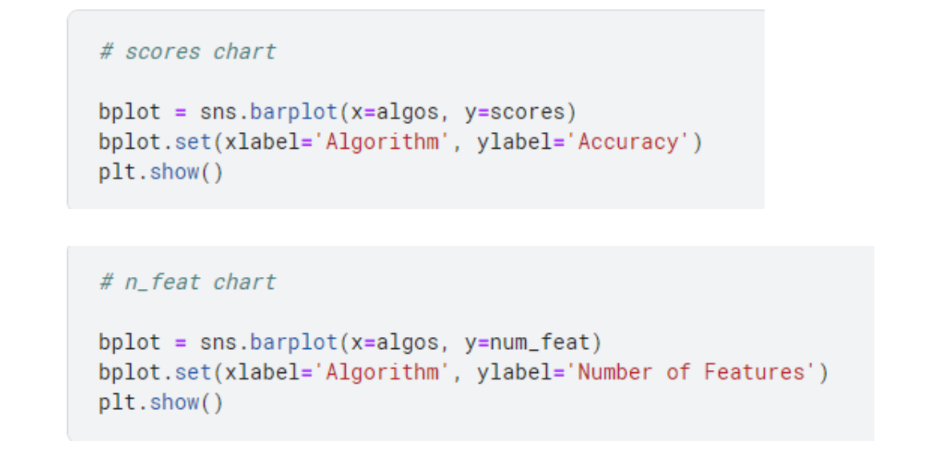
\includegraphics[width=6in]{images/c9.png} 
   \\\fontsize{11pt}{24pt} Code: Comparing number of features and accuracy
\end{center}

	 
		

\section{Final model and applying best metaheuristic}
We then compared the results of the various pre-trained models to select the best model and similarly compared different metaheuristics to select the best fit algorithms. We then trained an entirely new model based on the pre-trained model with the best results, but this time on the entire dataset of 120,000 images. This training was run for 15 epochs and 0.0001 learning rate initially, with the early stopping limit being 3 epochs and the learning rate reduction limit being 2 epochs, post which the model was fine tuned for another 10 epochs with a learning rate of 0.00001. We then applied the best metaheuristic, this time for 20 epochs with a population size of 30. This reduction was due to the larger nature of the training data which induced restrictions on the time we could run the model for. We used the same data pipelines we’d defined initially for this phase of training too. We finally saved the selection of features outputted by our chosen metaheuristic. 

We start with the modified training and testing sets. 

\begin{center}
   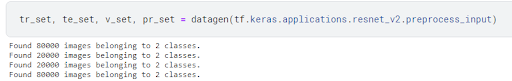
\includegraphics[width=6in]{images/c10.png} 
   \\\fontsize{11pt}{24pt} Code: Training on full dataset
\end{center}

		
  
We then modify training parameters.

\begin{center}
   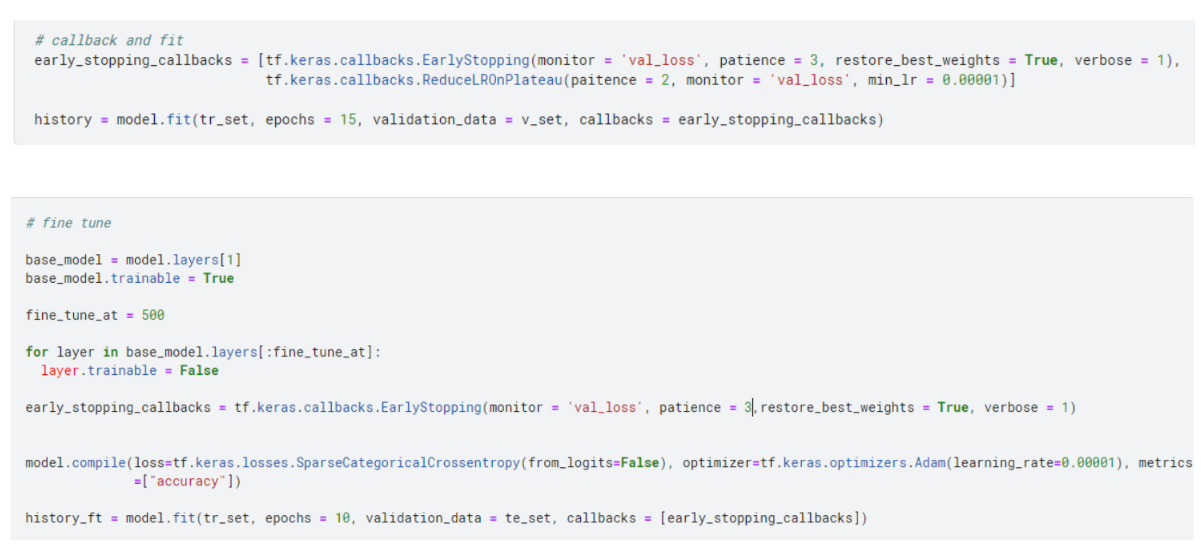
\includegraphics[width=6in,height=3in]{images/c11.png} 
   \\\fontsize{11pt}{24pt} Code: Modified training parameters
\end{center}
		
  
We lastly modify the run the code in figure (xix) to generate training and testing features and apply our metaheuristics with two modifications. Firstly, instead of using the KNN algorithm, we use a Multi-Layer Perceptron as our final classifier and secondly, we run the algorithms for only 20 epochs with a population size of 30.

\begin{center}
   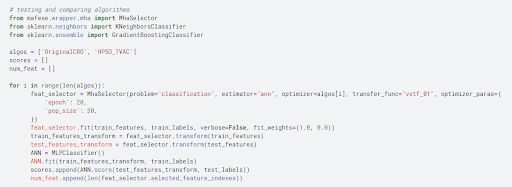
\includegraphics[width=6in, height=3in]{images/c12.png} 
   \\\fontsize{11pt}{24pt} Code: Final metaheuristic
\end{center}
		
		
  
We finally save the feature subset selected by our algorithm.


\begin{center}
   \includegraphics[width=5in]{images/c13.png} 
   \\\fontsize{11pt}{24pt} Code: Saving selected features
\end{center}
		
		
